\section{Related Works}

First of all, we need to go over some definitions for this part of our paper. In this section, we will be speaking of metrics, which are mesures of some property of a piece of software. There are several metrics that can be calculated in software, but we will mainly be talking about Ownership and Focus in the following sections.

\subsection{How Developers Drive Software Evolution}

This article was the one which introduced the notion of metric and Ownership to us. They analysed software repositories (CSV), in order to determine the Ownership of a file. They define the owner of a file as the developer with the highest amount of contributions to a file.
Determining ownership of a file may have many uses for software developers, but in this paper, they used this metric to create the following visualisation:\\
\\
\begin{figure}[p]
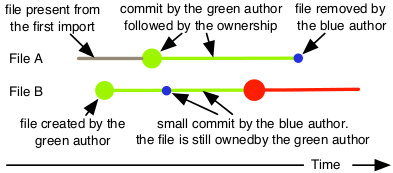
\includegraphics[width=0.5\textwidth]{./resources/girba2005.png}~
\caption{commit map}
\label{fig:commit_map}
\end{figure}

When this visualisation is applied to en entire, project, it becomes possible to detect behavioural pattern between developers. See annex[1].

\subsection{How Developers Develop Features}

In 2007 the same team published this paper, on a similar subject as the previous. This time, they focus is on the ownership of features, as well as files. The visualisation displays the ownership of files within the projects features, which are also structurally linked. The following image is a representation of this visualisation on a program that is designed to manage a mobile phone:\\
\\
\begin{figure}[p]
\centering
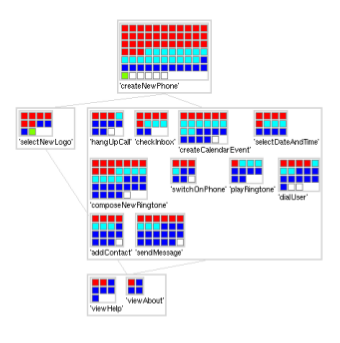
\includegraphics[width=0.4\textwidth]{./resources/girba2007.png}~
\caption{Ownership map By Feature}
\label{fig:ownership_map_by_feature}
\end{figure}

This visualisation makes it possible to determine who one might ask in order to help resolve a bug in a feature, rather than having to identify which file belong to which feature as one would need to do with the previous paper's visualisation[cite annex1].

\subsection{Dual Ecological Mesures in software development}

This paper took an interesting approach to mesuring focus in a software repository. Using a biological principal of prey/predator to refer to the relationship between components and developers. That is to say that modules prey on a developer's time. Therefore, in this visualisation, we have two points of view. On the one hand, the developers, and the contributions they have mande to each component (a larger edge represents more contributions), and on the other hand, we have the components, and the contributions they have received. As in the following figure:\\
\\
\begin{figure}[p]
\centering
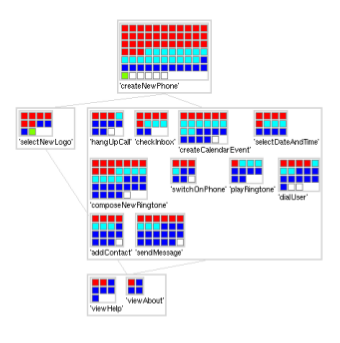
\includegraphics[width=0.4\textwidth]{./resources/girba2007.png}~
\caption{Ownership map By Feature}
\label{fig:ownership_map_by_feature}
\end{figure}

This is the visualisation that inspired us the most when deciding what kind of visualisation we should produce.